% !TeX root = ../main.tex

\section{Deterministic Demand Situation}
    \frame{\sectionpage}

    \begin{frame}{Seat Planning with Social Distancing}
      \begin{itemize}
      \item Group type $\mathcal{M} = \{1, \ldots, M\}$.
      \item Row $\mathcal{N} = \{1, \ldots, N\}$.
      \item The social distancing: $\delta$ seat(s).
      \item $n_i = i + \delta$: the new size of group type $i$ for each $i \in \mathcal{M}$.
      \item The number of seats in row $j$: $L_j^{0}, j \in \mathcal{N}$.
      \item $L_j = L_j^{0} + \delta$: the length of row $j$ for each $j \in \mathcal{N}$.
      \end{itemize}
      
      \begin{figure}[ht]
        \centering
        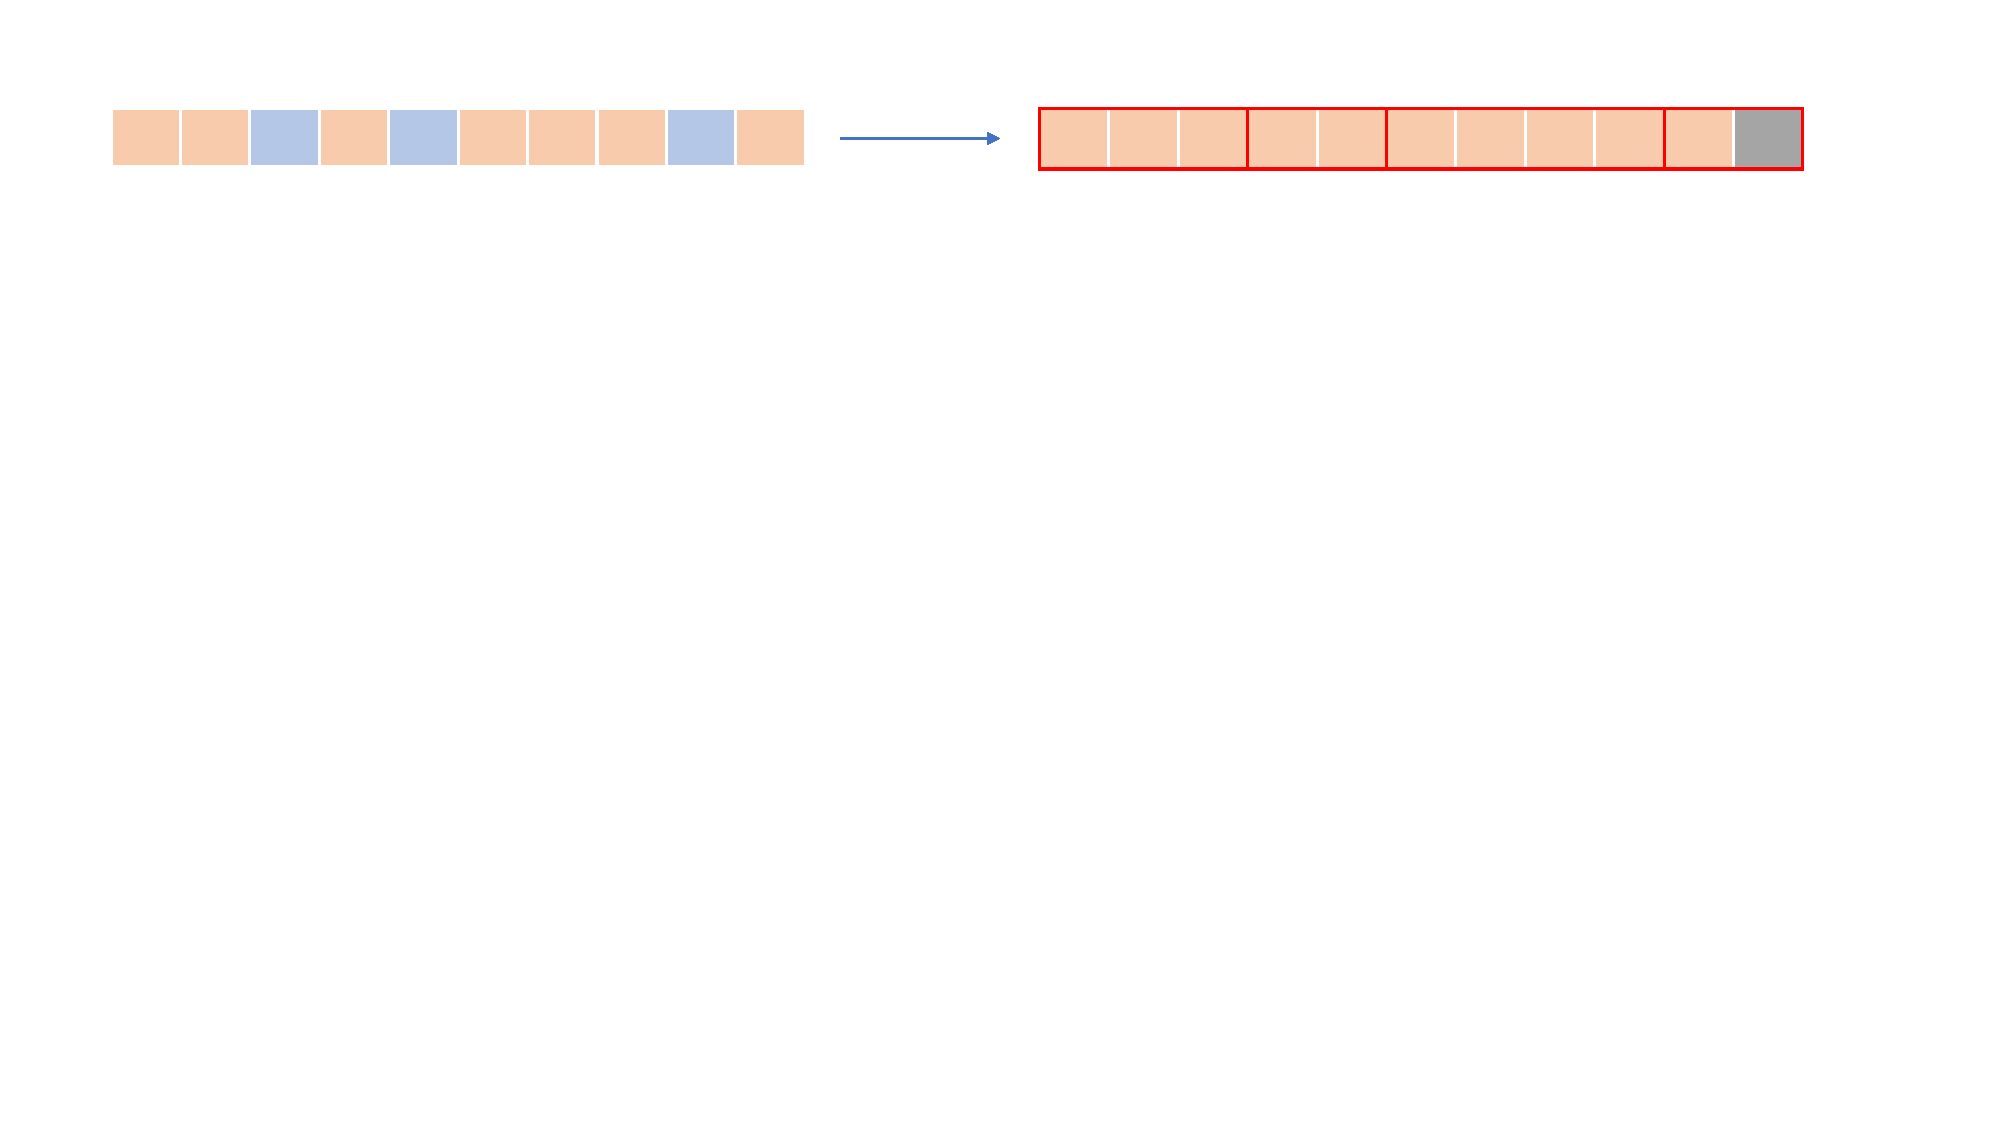
\includegraphics[width = 0.8\textwidth]{./images/dummy_seat.pdf}
        \caption{Problem Conversion with One Seat as Social Distancing}
    \end{figure}
    \end{frame}

  \begin{frame}{Basic Concepts}
    \begin{itemize}
      \item $\bm{h} = (h_1, \ldots, h_M)$, pattern, the seat planning for each group type in one row.
      Let $L = q(M + \delta) + r$.

      - The number of people accommodated: $|\bm{h}| = \sum_{i =1}^{M} i h_i = qM + \max\{r-\delta, 0\}$.
      
      - Loss for pattern $\bm{h}$: $L- \delta - |\bm{h}| = q \delta - \delta + \min\{r, \delta\}$.
      \item Largest patterns: $|\bm{h}| \geq |\bm{h}^{\prime}|$ for any $\bm{h}^{\prime}$. 
      \item Full patterns: $\sum_{i=1}^{M} n_i h_i = L$.
      \item[-] {\color{blue} Example}: 
      
      $\delta = 1$, $M =4$, $n_1 = 2, n_2 = 3, n_3 = 4, n_4 = 5$, $L = 21$.
      
      Largest patterns: $(0, 0, 0, 4), (0, 0, 4, 1), (0, 2, 0, 3)$.

      Largest may not be full: $(0, 0, 0, 4)$.

      Full may not be largest: $(1, 1, 4, 0)$.
    \end{itemize}
  \end{frame}

  \begin{frame}{Deterministic Formulation}  %开始一张幻灯片
    To obtain an integral seat planning, we use the deterministic formulation.
    
    \begin{equation}\label{deter_upper}
      \begin{aligned}
      \max \quad & \sum_{i=1}^{M}  \sum_{j= 1}^{N} (n_i- \delta) x_{ij} \\
      \text {s.t.} \quad & \sum_{j= 1}^{N} x_{ij} \leq d_{i}, \quad i \in \mathcal{M}, \\
      & \sum_{i=1}^{M} n_{i} x_{ij} \leq L_j, j \in \mathcal{N}, \\
      & x_{ij} \in \mathbb{Z}_{+}, \quad i \in \mathcal{M}, j \in \mathcal{N}.
      \end{aligned}
    \end{equation}
  
    Problem \eqref{deter_upper} can generate a feasible seat planning.
    
  \end{frame}

  \begin{frame}
    In the LP relaxation of problem \eqref{deter_upper}, there exists an index $v$ such that the optimal solutions satisfy the following conditions:

    \begin{itemize}
      \item For $i = 1,\ldots, v-1$, $x_{ij}^{*} = 0$ for all rows, indicating that no group type $i$ are assigned to any rows before index $v$.
      \item For $i = v+1,\ldots, M$, the optimal solution assigns $\sum_{j} x_{ij}^{*} = d_{i}$ group type $i$ to meet the demand for group type $i$.
      \item For $i = v$, the optimal solution assigns $\sum_{j} x_{ij}^{*} = \frac{L - \sum_{i = v+1}^{M} {d_i n_i}}{n_v}$ group type $v$ to the rows. This quantity is determined by the available supply, which is calculated as the remaining seats after accommodating the demands for group types $v+1$ to $M$, divided by the size of group type $v$, denoted as $n_v$.
    \end{itemize}
  \end{frame}

  \begin{frame}{Generate The Full or Largest Pattern}
    Given a specific pattern, we can convert it into a largest or full pattern while ensuring that the
    original group type requirements are met. When multiple full patterns are possible, our objective is to generate the pattern with minimal loss.

    Mathematically, for any pattern $\bm{h} = (h_1, \ldots, h_N)$, we seek to find a pattern $\bm{h}{'} = (h_1{'}, \ldots, h_N{'})$ that satisfies the following programming.

    \begin{equation}\label{full_largest}
      \begin{aligned}
      \max \quad & |\bm{h}{'}| \\
      \text {s.t.} \quad & h_1{'} \geq h_1 \\
      &  h_1{'} + h_2{'} \geq h_1 + h_2 \\
      & \cdots \\
      & h_1{'} + \ldots + h_N{'} \geq h_1 + \ldots + h_N.
      \end{aligned}
    \end{equation}
  \end{frame}
